\documentclass{article}

\usepackage[T2A]{fontenc}
\usepackage[utf8]{inputenc}
\usepackage[main=russian, english]{babel}

% Пакеты для работы с математикой
\usepackage{amsmath}
\usepackage{amsfonts}
\usepackage{amssymb}
\usepackage{mathtools}
\usepackage{relsize}
\usepackage{cancel}

% Пакет для описания псевдоалгоритмов
\usepackage{algpseudocode}
\usepackage{algorithm}

% Пакет для специальных символов
\usepackage{textcomp}

% Пакет для рисования диаграм
\usepackage{tikz}
% Для создания графов в 3 блоке
\usepackage[all]{xy}

% Пакет для вставки изображений
\usepackage{graphicx}
\graphicspath{{img/}}
\DeclareGraphicsExtensions{.pdf,.png,.jpg}

\usepackage[left=3cm, right=2cm, top=2cm, bottom=2cm]{geometry}
\pagestyle{plain}
\linespread{1.1} % Межстрочный интервал

\usepackage{indentfirst}
% ======================
% Данный файл должен содержать команды для упрощения написания текста
% Ниже вы найдете некоторый перечень комманд, которые я создал. На основе их можно создавать свои.
% ======================

% Красивые буквы
\newcommand{\N}{\mathbb{N}}
\newcommand{\Q}{\mathbb{Q}}
\newcommand{\Z}{\mathbb{Z}}
\newcommand{\K}{\mathbb{K}}
\newcommand{\R}{\mathbb{R}}

% Определения, утверждения, теоремы, замечания
\newcommand{\opr}{\emph{\textbf{Определение.}} }
\newcommand{\opri}{\emph{\textbf{\underline{Определение.}}} }
\newcommand{\utv}{\emph{\textbf{Утверждение.}} }
\newcommand{\utvi}{\emph{\textbf{\underline{Утверждение.}}} }
\newcommand{\thr}{\emph{\textbf{Теорема.}} }
\newcommand{\thri}{\emph{\textbf{\underline{Теорема.}}} }
\newcommand{\proof}{\emph{Док-во:} }
\newcommand{\lem}{\emph{\textbf{Лемма.}} }
\newcommand{\lemi}{\emph{\textbf{\underline{Лемма.}}} }
\newcommand{\note}{\emph{\textbf{Замечание.}} }
\newcommand{\notei}{\emph{\textbf{\underline{Замечание.}}} }
\newcommand{\conseq}{\emph{\textbf{Следствие.}} }
\newcommand{\example}{\emph{Пример.} }
\newcommand{\examplei}{\emph{\textbf{Пример.}} }

% Команда для отображения
\newcommand{\map}[3]{\ensuremath{#1: #2 \rightarrow #3}}


\title{Лекции по дискретной математике}
\date{\today}
\author{me and boyz}

\begin{document}
\maketitle
\tableofcontents

% ======= Лекция 1 ========
\section{Дискретные функции и их представление. Индуктивное определение формулы. Полные системы. Критерий полноты.}

\opr Дискретной функцией называется любая функция, отображающая конечное множество $A$ в конечное множество $B$.

Область определения дискретной функции часто представляется в виде декартового произведения множеств относительно небольшой мощности.

Если \map{f}{A}{B} - дискретная функция и $A = A_1 \times \ldots \times A_n$, то $f$ обозначают следующим образом $f(x_1;\dots;x_n)$ и называют
дискретной функцией от $n$ переменных $x_1,\dots,x_n$. При этом $x_i$ принимает всевозможные значения из $A_i$.
Если $A_1 = \ldots = A_n = B$ и $B = \{0, 1\}$, то $f$ называется булевой функцией.

\opr Обозначим далее $\Omega = \{0, 1\}$, тогда булевой функцией от $n$ переменных называется любое отображение \map{f}{\Omega^n}{\Omega}.

0-местными булевыми функциями будем называть элементы $0, 1 \in \Omega$.

\note Существуют функции $k$ - значной логики.

Обозначать булеву функцию будем $f(x_1;\dots;x_n)$ или $f(\vec{x})$, если количество переменных известно из контекста.

\opr Если $f(x_1;\dots;x_n)$ - булева функция и $\vec{\alpha} = (a_1; \dots; a_n) \in \Omega^n$, то образ $\vec{\alpha}$ при отображении
$f$ называют значением функции $f$ на наборе $\vec{\alpha}$. Обозначение: $f(\vec{\alpha})$.

\opr Если рассматривать 0 и 1 как числа $\in \N_0$, то для набора $\vec{\alpha} = (a_1; \dots; a_n)$ обозначим
$||\vec{\alpha}|| = a_1 + \ldots + a_n$ - вес вектора $\vec{\alpha}$.

$\widetilde{a} = \sum\limits_{i=1}^{n} a_i 2^{n-i}$ - лексикографический порядок.

\example
$$
\vec{\alpha} = (1; 1; 0; 1) \Rightarrow ||\vec{\alpha}|| = 1 + 1 + 0 + 1 = 3.
$$

Естественным образом задания является табличный, при этом координата $i$-вектора $f^{\downarrow}$ соответствует значению
$f(\vec{\alpha})$, где $\widetilde{a} = i$.

\example
$$
\begin{matrix}
    x_0 & x_1 & f^{\downarrow} \\
    0 & 0 & 0 \\
    0 & 1 & 1 \\
    1 & 0 & 1 \\
    1 & 1 & 1 \\
\end{matrix}
$$

\utv $|F_2(n)|= 2^{2^n}$.

\opr Весом булевой функции $f$ называют величину $||f|| = |\{\vec{\alpha} \in \Omega^n \mid f(\vec{\alpha}) = 1\}|$. $N_f$ - носитель булевой функции.

\opr Функция от $n-1$ переменной, определяемая равенством $\varphi(a_1; \dots; a_{n-1}) =$\\
$f'(a_1; \dots; a_{i-1}; b; a_{i+1}; \dots; a_n)$, называется
функцией полученной из $f'$ фиксацией $i$-ой переменной значением $b$.

Обозначением $\varphi = f_i^b(x_1; \dots; x_n)$, аналогично фиксация $k$ переменных значениями $b_1,\dots, b_k : \varphi = f_{i_1; \dots; i_n}^{b_1; \dots; b_k}(x_1; \dots; x_n)$.

Общее название таких функций $\varphi$ - подфункции $f$. 

Если $f(a_1; \dots; a_{i-1};0;a_{i+1}; \dots; a_n) = f(a_1; \dots; a_{i-1};1;a_{i+1}; \dots; a_n)$, $\forall a_1, \dots, a_{i-1}, a_{i+1}, \dots, a_n \in \Omega$, то 
переменная $x_i$ называется несущественной переменной функции $f$, в противном случае - существенной.

\opr Пусть $x_i$ -несущественная(\emph{фиктивная}) переменная функции $f$, $g$ получена из $f$ фиксацией $x_i$ любой константой, тогда говорят, что $g$
получена удалением из $f$ несущественной переменной $x_i$, а $f$ получена из $g$ добавлением фиктивной переменной $x_i$.

Пусть задано множество функций $\K = \{f_i : i \in I\}$ и множество символов переменных $X = \{x_1; \dots; x_n\}$.

\opr \begin{enumerate}
    \item Любой символ переменной есть формула над классом $\K$.
    \item Если $f_j$ - символ $m$ - местной функции из $\K$, а $A_1, \dots, A_m$ - формулы над $\K$, то $f_j(A_1; \dots; A_m)$ - формула над $\K$.
    \item Других формул нет.
\end{enumerate}

Множество формул над $\K$ обозначается $[\K]$. При $m=0$ формула есть символ над $\K$, т.е. константа.

\opr Число символов функций из $\K$, встречающихся в формуле $A$ назовем рангом формулы $A$. Обозначение: $r(A)$.

\opr \begin{enumerate}
    \item Подформула формулы $x_i$ - только она сама.
    \item Подформулы $f_j(A_1; \dots; A_n)$ - она сама и все подформулы формулы $A_1; \dots; A_n$.
\end{enumerate}

\opr Пусть $A$ - произвольная формула, в ее записи присутствует только переменные $x_{i_1}, \ldots, x_{i_k}$. Набор $x_{j_1}, \ldots, x_{j_m}$ называется
допустимым, если $\{x_{i_1}, \ldots, x_{i_k}\} \subseteq \{x_{j_1}, \ldots, x_{j_m}\}$.

Каждой формуле при фиксированном допустимом наборе $(x_1; \dots; x_n)$ сопоставляется функция по следующему правилу:
\begin{enumerate}
    \item Если $A$ есть $x_i$, то ей сопоставляется функция $f$, значения которой определяются равенством $f(a_1;\dots;a_n) = a_i, (a_1;\dots;a_n) \in \Omega^n$.
    \item Если $A$ есть $f_j(A_1;\dots; A_m)$ и формулам $A_1, \dots, A_m$ сопоставлены функции \\ $\varphi_1(x_1;\dots;x_n); \dots;\varphi_m(x_1;\dots;x_n)$, то формуле $A$ сопоставляется
функция $f$, значения которой определяются равенством $f(a_1;\dots;a_n) = f_j(b_1;\dots;b_m)$, где $b_\xi = \varphi_\xi (a_1;\dots;a_n), \xi \in \overline{1, m}$.
\end{enumerate}

\opr Формулы $A$ и $B$ равносильны, если они представляют одну и ту же функцию на любом допустимом наборе. Обозначение: $A\equiv B$.

\opr Пусть $A$ - произвольная формула над классом $\K = \{ \text{\&}, \vee, \bar{ } \}$. Двойственной к $A$ называется формула полученная из $A$ заменой $\text{\&} \leftrightarrow \vee$. Обозначение: $A^*$.

\thr $A^*(x_1; \dots; x_n) = \overline{A(\overline{x_1}; \dots; \overline{x_n})}$.

\conseq $A \equiv B \Leftrightarrow A^* \equiv B^*$.

\opr Замыканием системы $\K$ булевых функций называют множество всех булевых функций представимых формулами над $\K$. Обозначение: $[\K]$.

\utv \begin{enumerate}
    \item $\K \subseteq [\K]$
    \item $\K_1 \subseteq \K_2 \Rightarrow [\K_1] \subseteq [\K_2]$
    \item $[[\K]] = [\K]$
\end{enumerate}

\opr Система $\K$ называется полной, если (замыкание) $[\K] = F_2$.

\examplei
\begin{align*}
    \begin{rcases}
        \K_0 &= \{x_1 \cdot x_2; x_1 \vee x_2; \overline{x_1}\} \\
        \K_5 &= \{x_1 \cdot x_2; x_1 \oplus x_2; 1\}
    \end{rcases}
    \text{Полные}
\end{align*}

\opr Класс булевых функций называется замкнутым, если $\K = [\K]$.

Говорят, что набор $\vec{\beta}$ мажорирует набор $\vec{\alpha}$, если $\forall i \in \overline{1, n}: a_i \leq b_i$. Обозначение: $\vec{\alpha} \preccurlyeq \vec{\beta}$.

\examplei
\begin{align*}
    &T_0 = \{f(x_1; \dots; x_n) \mid f(0; \dots; 0) = 0\}\\
    &T_1 = \{f(x_1; \dots; x_n) \mid f(1; \dots; 1) = 1\}\\
    &L   = \{f(x_1; \dots; x_n) = a_1x_1 \oplus \ldots \oplus a_nx_n \mid a_i \in \Omega, i \in \overline{0, n}\} - \text{класс линейных функций}\\
    &S   = \{f(x_1; \dots; x_n) \mid f(x_1; \dots; x_n) \equiv \overline{f(\overline{x_1}; \dots; \overline{x_n})} \} - \text{класс самодвойственных функций} \\
    &M   = \{f(x_1; \dots; x_n) \mid \text{верно } \vec{\alpha} \preccurlyeq \vec{\beta}, \text{то} f(\vec{\alpha} \leq f(\vec{\beta})) \forall \vec{\alpha}, \vec{\beta} \in \Omega^n\} - \text{класс монотонных функций}
\end{align*}

\lem Булева функция $f(x_1; \dots; x_n)$ не является монотонной $\Leftrightarrow \exists \vec{\alpha}$ и $\vec{\beta}$ отличающиеся
только в одной координате (соседние наборы), такие что $\vec{\alpha} \preccurlyeq \vec{\beta}$ и $f(\vec{\alpha}) > f(\vec{\beta})$.

\thr $T_0, T_1, M, S, L$ - замкнуты.

\thr (Критерий Поста)

Система булевых функций $\K$ полна $\Leftrightarrow \K$ содержит функции из $F_2 \backslash T_0, F_2 \backslash T_1, F_2 \backslash M, F_2 \backslash S, F_2 \backslash L$.

\proof 

    $\underline{\text{Необходимость}}$

    $\forall$ произвольного замкнутого класса $G \neq F_2$, если $\K$ не содержит ни одной функции из $F \backslash G$, то $\K \subset G \Rightarrow [\K] \subset [G] \neq F_2 \Rightarrow \K$ - не
является полной.

    $\underline{\text{Достаточность}}$

    Рассмотрим функции $f_1 \notin T_0, f_2 \notin T_1, f_3 \notin L, f_4 \notin S, f_5 \notin M$.
    Покажем, что если $\K \nsubseteq G$, где $G \in \{T_0, T_1, S, M, L\}$, то $\overline{x}$ и $x_1\cdot x_2 \in [\K]$.

    Рассмотрим 2 случая:
    \begin{enumerate}
        \item $f_1(1; \dots; 1) = 1$, но тогда $f(x; \dots; x) = 1 \in [\K]$. Т.к. $\K \nsubseteq T_1$, то $\exists f_2 \in \K \mid f_2(1;\dots;1) = 0 \in [\K]$.
        Покажем, что $\overline{x} \in [\K]$. Т.к. $\K \nsubseteq M$, то $\exists f_3 \in \K \mid f_3 \notin M$, т.е. $\exists \vec{\alpha} \preccurlyeq \vec{\beta} \mid f_3(\vec{\alpha}) > f_3(\vec{\beta})$.

        Рассмотрим функцию $f_(a_1; \dots; a_{j-1}; x_j; a_{j+1}; \dots; a_n) \equiv \overline{x_j}$, т.к. 0 и 1 $\in [\K]$, то и $\overline{x} \in [\K]$.

        \item $f_1(1; \dots; 1) = 0$, то $f_1(x; \dots; x) = \overline{x} \in [\K]$. Покажем, что 0 и 1 $\in [\K]$.
        
        Рассмотрим $f_4 \in \K \mid f_4 \notin S \Rightarrow \exists (a_1; \dots; a_n) \mid f_4(a_1; \dots; a_n) = f_4(\overline{a_1}; \dots; \overline{a_n}) = const \in \{0,1\} \in [\K]$.
        Т.к. $\overline{x} \in [\K]$, то 0 и 1 $\in [\K]$.
    \end{enumerate}

    Покажем $x_1 \cdot x_2 \in [\K]$.

    Т.к. $\K \notin L$, то $\exists f_5 \in \K \mid f_5 \notin L$, т.е. в ее многочлене Жегалкина \emph{$\exists$ моном степени больше 1}(*) $\Rightarrow \exists$  моном, содержащий $x_1 \cdot x_2$.

    Рассмотрим многочлен Жегалкина функции $f_5$:
    $$
        f_5(x_1; \dots; x_n) = x_1 \cdot x_2 \cdot g_1(x_3; \dots; x_n) \oplus x_1 \cdot g_2(x_3;\dots;x_n) \oplus x_2 \cdot g_3(x_3; \dots; x_n) \oplus g_4(x_3; \dots; x_n).
    $$

    Рассмотрим функцию $f$, полученную из $f_5$, следующим образом:
    $$
    f(x_1; x_2) = f_5(x_1; x_2; a_3; \dots; a_n) = x_1x_2C_1 \oplus x_1C_2 \oplus x_2C_3 \oplus C_4.
    $$

    $C_1 = 1$, т.к. см (*). Рассмотрим функцию $f(x_1 \oplus C_3; x_2 \oplus C_2) = x_1x_2 \oplus C_2C_3 \oplus C_4 \Rightarrow x_1x_2 \in [\K]$. $\blacksquare$


\newpage
% =========================

% ======= Лекция 2 ========
\section {Классическое представление булевых функций. КНФ. ДНФ.}

Рассмотрим класс $K_0 = \{ \cdot , \vee , \bar{ }\}$
Символом $x^a$, где $a \in \Omega $, обозначим функцию переменной $x$, принимающую значение 1, если $x = a$, и 0 в противном случае. Таким образом:
\begin{center}
	\begin{equation*}
		x^a =
		\begin{cases}
   			$x, a = 1$
			\\
			\bar{x},a = 0
 		\end{cases}
	\end{equation*}
\end{center}

\opr
Пусть $i_1, \dotsc, i_k$ - различные натуральные числа. Формула вида $x_{i_1}^{a_1} \vee \dotsc \vee x_{i_k}^{a_k}$ называется элементарной дизъюнкцией ранга $k$.\par Если заменить $\vee$ на $\&$, то получаем элементарную конъюнкцию ранга $k$. \par Если элементраная дизъюнкция рассматривается как формула от переменной $x_1, \dotsc,x_n$ и её ранг равен $n$, то она назвается совершенной.

\opr Конъюктивной нормальной формой (КНФ) называется $\forall$ формула представляющая собой конъюнкцию конечного числа элементарных дизъюнкций.

\thr $\forall$ булевая функция может быть представлена в виде $f(x_1, \dotsc, x_n) = \Large\&\normalsize_{(b_1, \dotsc, b_k) = \Omega^k} x_{i_1}^{\bar{b}_{i_1}},\dotsc,x_{i_k}^{\bar{b}_{i_k}}f_{i_1, \dotsc, i_n}^{\bar{b}_{i_1},\dotsc,\bar{b}_{i_n}}(x_1,\dotsc,x_n)$ %оставь надежду, всяк сюда смотрящий

\note Аналогичным образом определяется элементарная дизъюнкция(ДНФ).

\thr $\forall$ булевой функции $k\leq n$ представима формулой $f(x_1,\dotsc,x_n) = \Large\vee\normalsize_{(a_1, \dotsc, a_k)} x_{i_1}^{a_{i_1}},\dotsc,x_{i_k}^{a_{i_k}}f_{i_1, \dotsc, i_n}^{a_{i_1},\dotsc,a_{i_n}}(x_1,\dotsc,x_n)$ %как и сюда

\conseq $f(x_1,\dotsc,x_n) \equiv \overline{x_1}f(0,x_2,\dotsc,x_n) \vee x_1f(1, x_2, \dotsc, x_n)$

В случае $k = n$ получаем совершенные КНФ и ДНФ, называемые СКНФ и СДНФ.

\utv $\exists!$ СДНФ и СКНФ $\forall f \in F_2$.

\example (две ДНФ одной функции) \par $\overline{x_1}\overline{x_2}x_3 \vee \overline{x_1}x_2x_3 \vee x_1x_2 \equiv \overline{x_1}x_3 \vee x_1x_2$

\opr Многочленом Жегалкина от переменных $x_1, \dotsc, x_n$ называется формула над классом $K_5=\{\oplus, \cdot, 1\}$ вида
\begin{center}
	$a_0 \oplus \sum_{i_1, \dotsc,i_k} a_{i_1, \dotsc, i_n}x_{i_1}\cdot \dotsc \cdot x_{i_n}$\\$1 \leq i_1 \leq \dotsc \leq i_k \leq n; a_0, a_{i_1}, \dotsc, a_{i_n} \in \Omega$
\end{center}
Здесь знак суммы означает исключающее "или" и сумирование ведётся по всем непустым подмножествам $\{i_1, \dotsc, i_k\}$ множества $\{1, \dotsc, n\}$.

\opr Элементарной конъюнкцией входящей в многочлен Жегалкина в качестве слогаемых называется одночлен (моном), элементы $a_{i_1, \dotsc, i_k}$ коэффиценты многочлена, $a_0$ - свободный член. Ранг конъюнкции называется степенью одночлена. \par Степенью неленейности функции представляемой многочленом Жегалкина называется максимальная из степеней многочлена, входящих в многочлен Жегалкина этой функции с коэффицентом 1.

\thr $\forall$ булевая функция однозначно представима многочленом Жегалкина.

\opr Двоичным n-мерным кубом называют множество точек пространства $\R^n$ с координатами $a_1, \dotsc, a_n$, где $a_i \in \Omega$

Для задания булевой функции $f(x_1,\dotsc,x_n)$ на n-мерном кубе отмечают вершины соответствующие носителю этой функции.

\opr Гранью n-мерного куба ранга $k$ (или иначе разморности $n-k$) называется множество его вершин, соответсвующее $N_{\varphi}$, где $\varphi$ - произвольная элементарная конъюнкция ранга k, т.е. $\varphi = x_{i_1}^{a_1}, \dotsc, x_{i_n}^{a_k}$

\utv(свойства)
\begin{enumerate} 
	\item $f = \varphi \Leftrightarrow N_f = N_{\varphi}$
	\item $N_{f \cdot \varphi} = N_f \cap N_{\varphi}$
	\item $N_{f \cup \varphi} = N_f \cup N_{\varphi}$
	\item $f \cup \varphi \equiv f \Leftrightarrow N_{\varphi}\subseteq N_f$
	\item $f \equiv \Large\vee_{i=1}^m\varphi_i \Leftrightarrow N_f = \Large\cup_{i=1}^mN_{\varphi_i}$
\end{enumerate}

\opr Длиной ДНФ называется сумма рангов входящих в неё элементарных конъюнкций. ДНФ с минимальной длиной называется минимальной ДНФ (МДНФ).

\opr Элементарная конъюнкция $\psi = x_{i_1}^{a_1}\cdot \dotsc \cdot x_{i_k}^{a_k}$ называется имплекантой функции $f(x_1,\dotsc,x_n)$, если она входит в некоторую ДНФ представляющуюю функцию f.

\utv (эквивалентно)
\begin{enumerate}
	\item $\psi$ - имплеканта функции f
	\item $\psi \cup f \equiv f$
	\item $\psi \rightarrow f \equiv 1$
	\item $\psi \cdot f = \psi$
\end{enumerate}

\opr Говорят, что g поглащается функцией f, если $g \vee f \equiv f$, т.е. имплеканта это элементарная конъюнкция, поглощаемая функцией f.

\opr Имплеканта функции f называется простой, если никакая её собственная часть не поглощается функцией f.

\example \\
$f(x_1, x_2, x_3) \equiv x_1x_2 \vee x_1\overline{x_2}\vee \overline{x_2} \overline{x_3}$\\
$\overline{x_2} \overline{x_3}$ - простая.\\
$x_1x_2$ - нет, т.к. $x_1$ поглощается f.

\lemma Пусть $\varphi_1$ и $\varphi_2$ имплеканты f, $\varphi_1$ поглощает $\varphi_2 \Leftrightarrow \varphi_1$ - часть $\varphi_2$

\thr $\forall$ имплеканта функции f, содержащаяся в какой-либо МДНФ функции f является простой.

\thr Пусть $\varphi_1 \cup\dotsc\cup \varphi_m$ - дизъюнкция всех простых имплекант функции f, тогда $f \leq \varphi_1 \vee\dotsc\vee \varphi_m$

\opr Дизъюнкция всех простых имплекант функции f называется сокращенной ДНФ.

\opr ДНФ $\varphi_1 \cup\dotsc\cup \varphi_m$ функции f называется тупиковой, если все $\varphi_i, i \in \overline{1, k}$, входящие в неё, являются простыми имплекантами f и $\varphi$.

Всюду далее $f-n$-местная булевая функция отличается от константы.

\section {Метод Блейка}
Метод Блейка строит из ДНФ сокращённую ДНФ.\par
Основной операцией данного алгоритма является операция неполного склеивания, в основе которого лежит тождество:
\begin{center}
	$x\varphi_1 \vee \bar{x}\varphi_2 \equiv x\varphi_1 \vee \bar{x}\varphi_2 \vee \varphi_1\varphi_2$
\end{center}
Вход: ДНФ\\
Выход: Сокращённая ДНФ

\underline{Этап 1}
В исходной ДНФ нааходим пару имплекант, в которой некоторая переменная входит в разных степенях: $\varphi_i = x_k\varphi_i'$ и $\varphi_j = \overline{x_k}\varphi_j'$.\par
Формируем $\varphi_1\varphi_2$ и добавляем её в ДНФ, повторяем до тех пор, пока не перестанут повялятся новые имплеканты.

\underline{Этап 2}
В полученной ДНФ применяем операцию поглащения используя тождество $\varphi\psi\vee\varphi\equiv\varphi$ до тех пор пока это возможно.

\thr Полученная на выходе алгоритма ДНФ является сокращённой ДНФ.

\proof Покажем, что ДНФ, полученная на \underline{Этапе 1} содержит все простые имплеканты функции f(индукция по n).\par
Пусть $n=1$. Утверждение очевидно, т.к. ДНФ функции одной переменной отличной от константы есть $x_1$ или $\overline{x_1}$.\par
Пусть $\forall$ ДНФ и для $\forall$ функции от n-1 переменной после \underline{Этапа 1} образуется ДНФ, содержащая все простые имплеканты.\par
Пусть теперь $f$ - функция от $n$ переменных и $\varphi$ её имплеканта 
\begin{itemize}
	\item[а)]Если ранг $\varphi$ равен n, то $\varphi$ содержится в $\forall$ ДНФ функции f.\par
Действительно пусть $\varphi = x_1^{a_1}\cdot \dotsc \cdot x_n^{a_n}$, тогда она принемает значения 1$\Leftrightarrow$ все $x_i$ равны $a_i$ в любой ДНФ функции f должна присутствовать имплеканта $\varphi'$, принимающая значение 1 на $(a_1, \dotsc, a_n) \Rightarrow$ все переменные входят в неё в тех же степенях, что и в $\varphi$, но
	\item[б)]Если ранг $\varphi$ меньше, то $\exists x_i$ не входящее в $\varphi$.\par
Представим f в виде $f=x_ih\vee \overline{x_i}g \vee t$, где $h,g,t$ - некоторые булевые функции, независящие от $x_i$. Т.к. $\varphi$ - имплекация функции f, то $\varphi\vee x_ih\vee \overline{x_i}g\vee t$ совпадает с $x_ih\vee \overline{x_i}g\vee t$. Полагая $x_i = 0$ или 1 имеем $\varphi\vee g\vee t\equiv g\vee t$ и $\varphi\vee h\vee t\equiv h\vee t$ соответственно. Возьмём конъюнкцию этих тождеств и применим к левой части закон дистрибутвности. Получим $\varphi\vee (g\vee t)(h\vee t) \equiv (g\vee t)(h\vee t) \Rightarrow \varphi$ является имплекантой функции $f_1=(h\vee t)(g\vee t)\equiv hg\vee t$.\par ДНФ этой функции получается с помощью операции "неполного склеивания" из имплекант, входящих в ДНФ функции $x_ih\vee \overline{x_i}g \vee t$. При этом $\varphi$ - простоая для f, т.к. $\varphi$ - простая для $f_1$, а f поглащает $f_1$.\par
Тогда по предположению индукции $\varphi$ содержится в ДНФ, полученной после \underline{Этапа 1}, применнёного к ДНФ функции $f_1$, но $\varphi \in$ аналогичной ДНФ функции f, т.к. $\forall$ непростая имплеканта поглащается некоторой простой, то после \underline{Этапа 2} в ДНФ окажутся только простые имплеканты.
\end{itemize}

\lemma Путь ДНФ $A = \Large\cup_{i=1}^k\varphi_i$ поглащает элементарную конъюнкцию $\varphi$ и $\varphi \varphi_k \equiv 0$. Тогда $\varphi$ поглащается ДНФ $A^1=\Large\cup_{i=1}^k\varphi_i$

\opr Функции $f_1$ и $f_2$ называются ортогональными, если $f_1f_2 \equiv 0$

\thr(Критерий поглощения)\par
Пусть  $A=\Large\cup_{i=1}^k\Large u_i$ - ДНФ некоторой функции, $\varphi_0$ - элементарная конъюнкция не ортогональная ни одной из конъюнкций $\varphi_1, \dotsc,\varphi_k$. Обозначим $\varphi_{0_i}$ - конъюнкцию членов входящих в $\varphi_0$  и в $\varphi_i$, а $\varphi_{1_i}$ - конъюнкция членов $\varphi_i$, невходящих в $\varphi_0$ (если $\varphi_i = \varphi_{0_i}, \varphi_{1_i} = 1$) ДНФ поглощает $\varphi \Leftrightarrow \Large\vee_{i=1}^k\varphi_{1_i} \equiv 1$

\utv Если f монотонна, то сокращённая ДНФ = МДНФ.

\section {Метод Квайна}
Составляется таблица, строчки которой обозначают всеми простыми имлекантами длиной функции, столбцы - наборами, на которых функция принимает значение 1. На пересечении ставится значение имплеканты на соответствующем наборе. Для построения ДНФ или МДНФ надо удалять строки так, чтобы в каждом столбце была хотя бы одна 1.

\end{document}	

\newpage
% =========================

% ======= Лекция 3 ========
 \section{Эквивалентность функций относительно групп преобразований.}

\subsection{Группы инерции}

\opr Подстановкой непустого множества $M$ называют любое биективное отображение $M$ на себя.
При известном n будем обозначать: $f(x_1; \ldots, x_n)=f(\vec{x})$.

\opr Пусть $f(\vec{x})$ и $h(\vec{x})$ - функции из $F_k(n)$ и $G$ - произвольная группа подстановок множества $\Omega_k^n$.
Говорят, что $f$ эквивалентно $h$ относительно группы $G$, если существует подстановка $g \in G \mid \forall \vec{\alpha} \in \Omega_k^n$ выполняется:
$$
f(\vec{\alpha})=h(g(\vec{\alpha})).
$$
Обозначение : $f \stackrel{G}{\sim} h$.
 
\utv
\begin{enumerate}
  \item $f \stackrel{G}{\sim} f$
  \item $f \stackrel{G}{\sim} h \Leftrightarrow h \stackrel{G}{\sim} f$
  \item $f \stackrel{G}{\sim} h, \  h \stackrel{G}{\sim} r \Rightarrow f \stackrel{G}{\sim} r$
\end{enumerate}

$\stackrel{G}{\sim}$ - отношение эквивалентности.

Таким образом $F_k(n)$ разбивается на классы эквивалентности. Класс, содержащий функию $f$, будем называть $[f]_G$.
Очевидно $1 \leq |[f]_G|\leq|G|$.

\opr Функция $f(\vec{x}) \in F_k(n) $ - называется инвариантной относительно подстановки $g \in G < S_{\Omega_k^n}$,
если $f(g(\vec{x})) = f(\vec{x})$, относительно группы $G$, если она инвариантна относительно любой подстановки из этой группы.

\utv Множество подстановок $g \in G$, относительно которых функция $f$ инвариантна образует подгруппу в группе $G$.

\opr Подгруппа, определенная в утверждении, называется - \emph{Группа инерции - функции $f$ в группе $G$}. Обозначение: $I_G(f)$.

\thr Если $f\in F_k(n)$ и $G < S_{\Omega^k}$, то $|[f]_G|=\frac{|G|}{|I_G(f)|}$

\opr Орбитой группы подстановок $G < S_{\Omega^k}$, содержащей элемент $\alpha$, называется множество
$$
\bigtriangleup_\alpha = \{ \beta \in \Omega_k^n\: |\:  \exists g\in G \mid \beta =g(\alpha)\}.
$$

\utv $f$ инвариантна относительно группы $G \Leftrightarrow$ на элементах каждоой орбиты она принимает постоянные значения.
То есть $\forall p \in \bigtriangleup_{\alpha} \mid f(\beta) = f(\alpha)$.

\conseq $G$ - транзитивна $\Leftrightarrow f$ инвариантна $\Leftrightarrow f \equiv$ const.

\conseq Число функций $k$ - значной логики инвариантных относительно группы $G$ равно $k^{\nu(G)}$, где $\nu(G)$ - число орбит группы $G$.

\examplei
\begin{enumerate}
  \item Группа подстановок координат векторов $\alpha \in \Omega_k^n$:
    \begin{align*}
      g_s(a_1, \dots , a_n)  =  a_{i_1};\dots ;a_{i_n} \text{в соответсвии с перестановкой}\  
      g_s=
      \begin{pmatrix}
        1 & \ldots & n \\
        i_1 & \ldots & i_n
      \end{pmatrix}
  \end{align*}
  Обозначение: $S_n$.

  \item Группа сдвигов: $\Sigma_n $. Пусть $\alpha = (a_1;\dots;a_n) \in \Omega_k^n $, тогда
    $$
      \Sigma_n = \{g_\alpha \mid g_\alpha(c_1; \ldots; c_n)=(c_1+a_1; \ldots; c_n+a_n); \alpha, \vec{c} \in \Omega_k^n\}
    $$
  Суммирование ведется по модулю $k$.

  \item Группа Джевонса $Q_n$:
    $$
      Q_n = <\Sigma_n;S_n>.
    $$
  \item $GL(n;k)$ - полная линейная группа. Пусть $A$ - невырожденная матрица размеров $n \times n $ над $\Z_k$, тогда
  $$
    GL(n;k)=\{q_A \mid q_A(a_1;\ldots;a_n) = (a_1;\ldots;a_n) \cdot A; A \in (\Z_k)_{n \times n}^* \}
  $$

  \item Полная афинная группа $AGL(n;k)=<GL(n;k);\Sigma_n>$.
\end{enumerate}

Диаграмма вложения группы:
\begin{align*}
  \xymatrix{
    S_n      \ar[r] \ar[rdd]  & GL(n; k) \ar[rd] \\
    & & AGL(n;k) \\
    \Sigma_n \ar[r]  & Q_n \ar[ru]
  }
\end{align*}

$\Sigma_n; Q_n; AGL(n;k) $ - транзитивные $\Rightarrow$ инвариантны относительно них только константы.

Орбитами группы $S_n$ являются множества векторов одинакового веса. Число функций одинакового веса инвариантных относительно$ S_n$ ровно $k^{k+n-1 \choose k-1}$.

\thr Орбитами группы $GL(n;k)$ являются все множества $M_\alpha=\{(a_1;\dots;a_n)\in \Omega_k^n|\mathrm{\text{НОД}}(a_1;\dots;a_n;k)=d\}, \text{где}\   d|k$.
                   
\conseq Число функций $n$ - значной логики (от $n$-переменных), инвариантных относительно $GL(n;k)$ равно $k^{\nu(k)}$,где $\nu(k)$ - число делителей $k$.

\thr
Пусть $T_k(n)$-множество всех функций $k$-значной логики с тривиальной группой инерции в $AGL(n;k)$. Тогда
$$
\lim_{n\to\infty} \frac{|T_n(k)|}{|F_k(n)|}=1.
$$

\proof
1) Оценим сверху число неподвижных точек нетождественного aфинного преобразования $g \in AGL(n;k)$.  Рассмотрим уравнение $g(\vec{x})=\vec{x}A+\alpha;\alpha \in Z_k^n;$ $A$-невырожденная матрица над $Z_k;$ В матричном виде уравнение перепишется следующим образом:\\
$\vec{x}(E-A)=\alpha. $\\
Если $A=E$ ,то $\nexists$ решений, так как $\vec{\alpha}\neq \vec{0}$ ($g$ - нетождественное преобразование). Пусть $ C=(C_{ij})_{n \times n} = E-A \neq 0 $.

Не ограниченная общность $c_{11} \neq 0 $ , тогда $ c_{11} x_1 + \ldots + c_{n1} x_n = a_1 $ -слогаемые системы, если зафиксировать $x_2;\dots;x_n $ произвольными значениями из $Z_k $, то полученное уравнение будет иметь не более $НОД(C_n;k) $ решений, а так как $C_{11} \neq 0$, то число решений при произвольной фиксации $x_2;\dots;x_n \leqslant \frac{k}{2} \rightarrow $ для всего уравнения имеем $ (\frac {k}{2})^n$. ( то есть число решений $\vec{x}(E-A) = \alpha $, не превосходит $(\frac {k}{2})^n \leqslant \frac {k^n}{2} $.)\\
2) Поскольку количество точек (неподвижных) афинной подстановки ( $ k^{l(g)} $, где $l(g)$-число циклов ) не превосзодят $\frac {k^n}{2} $, то количество независимых циклов в её разложении может превосходить $\frac {3k^n}{4} $. ( $\frac {k^n}{2} $ - циклов длины 1; $\frac {k^n}{4} $ - циклов длины 2)\\
$\rightarrow $ количество функций инвариантных относительно фиксированных подстановок $g$ не провосходят $k^{\frac{3k^n}{4}}$, так как функция должна принимать одинаковые значения на элементах каждой орбиты. \\
3) $$
|AGL(n;k)| \leqslant k^{n^2+n} \rightarrow k^{\frac{3k^n}{4} +n^2 +n} \rightarrow \lim_{n\to\infty} \frac{|T_n(k)|}{|F_k(n)|} = \frac {k^{k^n}-k^{\frac {3k^n}{n}+n^2+n}}{k^{k^n}}=1
$$

Классы эквивалентности по $\stackrel{G}{\sim}$ назовем $G$-типом. Для осуществления полной классификации необходимо построить список представителей $G$ типов.
$f^{(1)};\dots; f^{l(G)}; l(g)$- число $G$-типов.
Строится последовательность $f_1;f_2;\dots $. Среди них могу быть одинаковые представители из какого-то класса. Полагаем $ f^{(1)}=f_1$ и считаем:\\ 
$|I_G(f^{(1)})|$, проверяем $f_2 \in I_G(f^{(2)})$; если нет, то считаем:\\
$|I_G(f^{(2)})|, при f^{(2)} =f_2$ и так далее $\dots$\\
Останавливаемся, когда :\\
$$
\sum_{i=1}^{l} \frac{|G|}{|I_G(f^{(2)})|} = k^{k^n}
$$\\ то есть необходимость вычисления порядка групп инерции. Значение параметра $l(G)$ упрощает метод. Задача поиска этого параметра носит название задачи перечисления $G$ - типов.\\

\subsection{Инварианты, нахождение групп инерции и проверка экваивалентности.}

\opr 
Отображение $\varphi$ - называется инвариантом группы $G$, если для любого $g \in G$ и произвольной $m \in M$ справедливо равенство:\\
$\varphi(g(m))=\varphi(m)$.

Инвариант $\varphi$ называется полным, если из $\varphi (m_1) = \varphi(m_2) \Rightarrow $ что элементы $m_2 $ и $m_2$ лежат на одной орбите группы $G$. Принимая во внимание факт, что для $G$, действующей на $F_k(n)$, орбита будет являться $G$ - типом, сформируем правило проверки эквивалентности $f_1 $ и $f_2 \in F_k(n)$.\\
Пусть $\varphi$ - инвариант группы $G$, действующей на $F_k(n)$, если $\varphi$ -полный, то $\varphi(f_1)=\varphi(f_2) $ равносильно тому, что $f_1 \stackrel{G}{\sim} f_2$;\\
Если $\varphi$ неполный инвариант, то $\varphi(f_1)=\varphi(f_2) $ - только необходимое условие эквивалентности.
В случае, когда равенство выполнено, надо проверять другие инваринты:\\

$\sqsupset k = 2$
\begin{enumerate}
	\item Для $AGL(n;k); S_n; \sum_n; Q_n $ инварианты - вес, степени нелинейности.
	\item $Q_n$ - число простых импликант, число существенных переменных.
	\item $S_n$ - число одночленов в многочлене Жегалкина.\\
\end{enumerate}

\examplei
Пусть $f(x_1;x_2;x_3) = x_1\oplus x_2, f_2(x_1;x_2;x_3)=x_1 \oplus x_2 \oplus x_3$

Они не эквивалентны относительно $S_n;Q_n$, но
$f_2(x_1;x_2;x_3)=f_1((x_1;x_2;x_3)A)$\\

$A=
\begin{pmatrix}
  1 & 0 & 0\\
  0 & 1 & 0\\
  1 & 0 & 1
\end{pmatrix}$\\

\thr
Для любого натурального $ m \geqslant 2$ и произвольной группы $G$:
$|G|=m, \exists n\  \text{и}\  f\in F_2(n) \mid I_{S_n}(f) \cong G$.
 \newpage
% =========================

% ======= Лекция 4 ========
\section {Представление дискретных функций в базисах функциональных пространств. Алгоритм БПФ. }

\opr Пусть K - произвольное поле, 0 и 1 - нуль и единица поля K  соответствует псевдобулевой функции от n переменных называется произвольное отображение $f:\{0,1\}^{n} \longrightarrow K$.
Обобщение $ GF(p)^n \longrightarrow K$.
Множества таких функций будем называть $K_p(n)$. На $K_p(n)$ естественным образом задаются операции + и $\cdot$ на элементах поля.

\utv $K_p(n)$ - векторное пространство над $K$ размерности $p^n$

\thr Множеству всех различных гомоморфизмов $\varphi: (GF(p)^n,+) \longrightarrow (\mathbb{C},*)$ состоит из $p^n$ различных гомоморфизмов $\X_\alpha$; $\alpha = (\alpha_1,\dots, alpha_n) \in GF(p)^n$, каждый из которых однозначно определяется своим действием на вектора стандартного базиса $e_j, j \in \overline{1, n}$
следующим образом $\X_\alpha(e_j) = \exp(\frac{2\pi i}{p}\cdot \alpha_i).$

\utv Для любых $\alpha,\beta \in GF(p)^n$ верно $\frac{1}{p^n}\sum_{\gamma \in GF(p)^n}^n \X_\alpha (\gamma) \overline {\X_\beta (\gamma )} = \delta_{\alpha,\beta}$, т.е.
\begin{align*}
    \delta_{\alpha, \beta} = 
    \begin{cases}
        1, \alpha = \beta \\
        0, \alpha \neq \beta
    \end{cases}
\end{align*}

\thr $\{ \X_\alpha \mid \alpha \in (GF(p))^n \}$ - базис $\C_p(n)$

\opr Разложение произвольной функции $f \in \C_p(n)$ по базису характера $\{ \X_\alpha \mid \alpha \in (GF(p))^n \}: f(\vec{x}) =  \sum_{\alpha \in GF(p)^n} C_\alpha^f \X_\alpha(\vec{x})$ называется разложением $f$ в ряд Фурье, соответствующий набору $\alpha$. Комплексное число $C_\alpha^f$ - коэффициент Фурье функциий $f$
соотвествующий набору $\alpha$.

\opr Преобразование из $\C_p(n)$ в $\C^{p^n}$, ставящее в соответствие каждой функции ее коэффициенты Фурье(<<Спектр Фурье>>), будем называть преобразование Фурье.

\utv
\begin{enumerate}
    \item Пусть $\gamma \in GF(p)^n$, тогда $C_\gamma^f = \frac{1}{p^n}\sum_{\beta \in GF(p)^n} f(\beta) \overline{\X_\alpha(\beta)}$.
    \item Пусть $f$ - булева функция, тогда $C_\gamma^f = \frac{1}{2^n}||(f(\overline{x})||$.
\end{enumerate}

В некоторых случаях вместо функции $f$ удобнее свойства функции $F(\vec{x}) = (-1)^{f(\vec{x})}.$ Коэффиценты Фурье такой функции называется коэффициентом Уолша-Адамара второго рода функции $f(x)$. Обозначается $C_\alpha^F = W_\alpha^f$.\\

\prop
\begin{enumerate}
    \item $W_\alpha^f = 1 - \frac{1}{2^{n-1}} ||f(\vec{x}) \oplus  <\alpha,\vec{x}>||$, где $<\alpha, \vec{x}> = \alpha_1 x_1 \oplus \dots \oplus \alpha_n x_n$.

    \item \begin{align*}
            W_\alpha^f =
                \begin{cases}
                    -2 C_\alpha^f  : \alpha \neq \vec{0}\\
                    1-2 C_\alpha^f : \alpha = \vec{0}
                \end{cases}
            \end{align*}
    
    \item $\sum_{\alpha \in \Omega_2^n} W_\alpha^f = (-1)^{f(\overline{0})} $

    \item $\sum_{\alpha \in \Omega_2^n} (W_\alpha^f)^2 = 1$

    \item $\frac{1}{2^{\frac{n}{2}}} \leq \max_{\alpha \in \Omega_2^n} |W_\alpha^f| \leq 1$
\end{enumerate}

Зафиксируем некоторую обратимую $2^n \times 2^n$ матрицу $A$ над полем $K$. Пусть $f^{\downarrow}$ - вектор столбцов значений $f$ из $K_2(n)$.
$\widetilde{f^\downarrow} = A^{-1} f^\downarrow$, тогда задано биективное отображение из $K_2(n)$ в $K^{2^n}$.
Вектор $\widetilde{f^\downarrow}$ - представление функции $f$.
Если столбцы матрицы $A$ занумеровать наборами из $\Omega_2^n$, то $f^\downarrow = \sum_{\alpha \in \Omega_2^n} g_\alpha^\downarrow \widetilde{f}(\alpha)$.
Каждый столбец $g_\alpha^\downarrow$ есть задание некоторой функции из $K_2(n)$, $A$ - невырожденная $\Rightarrow \{ g_\alpha \}_{\alpha \in \Omega_2^n}$ - базис $K_2(n)$.

\opri Пусть $A$ и $B$ - матрицы над размеров $m \times n$ и $n \times n$ над полем $K$ соответственно. Тензорным произведением матриц $A$ и $B$ называется матрица $С = A \otimes B$ следующего вида:
\begin{align*}
    C =
    \begin{pmatrix}
        \alpha_{11}\beta & \alpha_{12}\beta & \dots & \alpha_{1m}\beta \\
        \vdots & \vdots & \ddots  & \vdots \\
        \alpha_{m1}\beta & \alpha_{m2}\beta & \dots & \alpha_{mn}\beta
    \end{pmatrix}
    - \text{размерность}\  mn \times mn.
\end{align*}

\utv
\begin{enumerate}
    \item $A \otimes (B \otimes C) = (A \otimes B) \otimes C$
    \item $(A + B) \otimes C = A \otimes C + B \otimes C $ ($m = n$) \\
          $A \otimes (B + C) = A \otimes B + A \otimes C $
    \item $A,C  \in K_{m;m}, B,D \in K_{n;n} \Rightarrow (A \otimes B)(C \otimes D) = AC \otimes BD$
    \item $A \oplus B$ обратимо $\Leftrightarrow$ $A$ и $B$ обратимы, причем $(A \otimes B)^{-1} = A^{-1} \otimes B^{-1}$
\end{enumerate}

\lem Пусть $A$ - матрица размера $2^n \times 2^n$ над $K$ и $A = B \otimes A'$, где $B = \begin{pmatrix}
    a & b\\
    c & d
\end{pmatrix}$
, $a,b,c,d \in K$, а $A$ - матрица размером $2^{n-1} \times 2^{n-1}$ причем обе матрицы $B$ и  $A'$ невырожденные.
Пусть столбцы матриц $A$ и $A'$ задают базисы функциональных пространств $K_2(n), K_2(n-1)$, функции из которых обозначаются $g_\alpha$ и ${g'}_\alpha$ соответственно.
Тогда $\forall \alpha \in \Omega_2^{n-1}$ верно:

$g_\alpha(0, \alpha') = (a \overline{x_1} + c x_1)g_{\alpha'}(x_2; \dots ;x_n)$\\
$g_\alpha(1, \alpha') = (b \overline{x_1} + d x_1)g_{\alpha'}(x_2; \dots ;x_n)$.

\thr Пусть A - тензорное произведение матриц $B_j \in K_{2\times2}^*$ вида $\begin{pmatrix}
    a_i & b_i\\
    c_i & d_i
\end{pmatrix}$,
т.е. $A = \otimes \prod_{i = 1}^n B_i$, тогда базисная функция $g_\omega$, соотвествующая столбцу $A$ и занумерованная набором $\omega = (\omega_1, \dots, \omega_n)$ имеет вид
$g_\omega(x_1; \dots; x_n) = \prod_{i=1}^n \omega_i(a_i\overline{x_i} + c_ix_i) + \omega_i(b_i\overline{x_i} + d_ix_i)$.

\example
\begin{align*}
    B = 
    \begin{cases}
        1 & 0\\
        0 & 1
    \end{cases}
    - \text{тождественное преобразование}.
\end{align*}

\begin{align*}
    B = 
    \begin{cases}
        1 & 0\\
        1 & 1
    \end{cases}
    - \text{многочлен Жегалкина}.
\end{align*}

\begin{align*}
    B = 
    \begin{cases}
        1 & 1\\
        1 & -1
    \end{cases}
    - \text{коэффициент Фурье}.
\end{align*}

\thr Пусть $B$ - невырожденная матрица размера $2 \times 2$  над $K$, $A = B^{[n]}$ - тензорная степень. Тогда существует алгоритм вычисления $\widetilde{f}^\downarrow$ по вектору $f^\downarrow$, имеющий сложность $O(n \cdot 2^n)$ операций поля $K$)\\

\proof Пусть $B^{-1} = $ $\begin{pmatrix}
        a & b\\
        c & d
    \end{pmatrix}$.
Из свойств тензорного произведения матриц вытекает, что $A^{-1} = (B^{-1})^{[n]}= D_n \cdot D_{n-1} \cdot \ldots \cdot D_1$, где $D_i$ - матрица вида:

\begin{align*}
    D_i = \left( E_2^{[n-i]} \otimes
    \begin{pmatrix}
        a & b\\
        c & d
    \end{pmatrix}
    \otimes E_2^{[i-1]} \right), \text{где}\  E_2 = 
    \begin{pmatrix}
        1 & 0 \\
        0 & 1
    \end{pmatrix}.
\end{align*}

Обозначим $f_0^\downarrow = f^\downarrow$ и $\forall i \in \overline{1,n} \mid f_i^\downarrow = D_i \cdot f_{i-1}^\downarrow$, тогда $\widetilde{f^\downarrow} = f_n^\downarrow$.

Покажем, что каждое из умножений $D_i$ на $f_{i-1}^\downarrow$ может быть выполнено за $O(2^n)$ операций поля $K$. Тогда общее количество операций, 
необходимое для вычисления $\widetilde{f^\downarrow}$ по $f^\downarrow$ будет составлять $0(n2^n)$ операций.

\begin{align*}
    D = \left( E_{2^{n-i}} \otimes
    \begin{pmatrix}
        aE_{2^{i-i}} & bE_{2^{i-i}}\\
        cE_{2^{i-i}} & dE_{2^{i-i}}
    \end{pmatrix}
    \right)
    =
    \begin{pmatrix}
        \hatv{D}_i &  & 0 \\
        & \ddots & \\
        0 & & \hatv{D}_i
    \end{pmatrix}
\end{align*}

$\hatv{D}_i$ - матрица размера $2^i \times 2^i$ вида
\begin{align*}
    \begin{pmatrix}
        aE_{2^{i-1}} & bE_{2^{i-1}}\\
        cE_{2^{i-1}} & dE_{2^{i-1}}
    \end{pmatrix}.
\end{align*}

Пусть теперь $X^\downarrow$ произвольный вектор длины $2^n$ над полем $K$. Опишем алгоритм умножения $D_i$ на $X^\downarrow$.

\begin{enumerate}
    \item Разобьем $X^\downarrow$ на $2^{n-1}$ частей длины $2^i$, тогда
        \begin{align*}
            X^\downarrow =
            \begin{pmatrix}
                X_1^\downarrow \\
                \vdots \\
                X_{2^{n-i}}^\downarrow
            \end{pmatrix}
            , \text{тогда}\  
            D_iX^\downarrow =
            \begin{pmatrix}
                \hatv{D}_iX_1^\downarrow \\
                \vdots \\ 
                \hatv{D}_iX_{2^{n-i}}^\downarrow
            \end{pmatrix}.
    \end{align*}

    \item Каждый из векторов $X_j^\downarrow$ разбиваем на 2 подвектора равной длины.
        \begin{align*}
            X_j^\downarrow &=
            \begin{pmatrix}
                X_{j_0}^\downarrow \\
                X_{j_1}^\downarrow
            \end{pmatrix}
            , \text{тогда}\  
            D_iX_j^\downarrow =
            \begin{pmatrix}
                aE_{2^{i-1}} & bE_{2^{i-1}}\\
                cE_{2^{i-1}} & dE_{2^{i-1}}
            \end{pmatrix}
            \begin{pmatrix}
                X_{j_0}^\downarrow\\
                X_{j_1}^\downarrow
            \end{pmatrix}
            = \\
            &=
            \begin{pmatrix}
                aE_{2^{i-1}}X_{j_0}^\downarrow + bE_{2^{i-1}} X_{j_0}^\downarrow \\
                cE_{2^{i-1}}X_{j_1}^\downarrow + dE_{2^{i-1}} X_{j_1}^\downarrow
            \end{pmatrix}
            =
            \begin{pmatrix}
                aX_{j_0}^\downarrow + bX_{j_0}^\downarrow\\
                cX_{j_1}^\downarrow + dX_{j_1}^\downarrow
            \end{pmatrix}.
        \end{align*}
\end{enumerate}

Таким образом для вычисления $\widetilde{f^\downarrow}$ необходимо $O(n \cdot 2^n)$ операций.
\newpage
% =========================

% ======= Лекция 5 ========
\section{Трансверсали.}

\opri Пусть $2^{X}$ - булеан множества $X$, т.е. совокупность всех подмножеств множества $X$. Пусть $(X_1; \dots; X_n)$ - некоторая $n$-выборка из булеана. Вектор $(x_1; \dots; x_n)$, состоящий из элементов множества $X$, называется трансверсалью семейства $(X_1; \dots; X_n)$, если выполнены следующие отношения:

\begin{enumerate}
\item $x_i \in X_i$ ; $1 \leq i \leq n$;
\item $x_i \neq x_j$ ; $i \neq j$; $1 \leq i$, $j \leq n$.
\end{enumerate}

Иными словами имеем систему различных представителей семейства $(X_1; \dots; X_n)$ .\\
Обозначается $(x_1; \dots; x_n)$ тр. $(X_1; \dots; X_n)$

\thr \textbf{(Критерий Ф.Холла)}
Для того, чтобы семейство $(X_1; \dots; X_n)$ имело трансверсаль, необходимо и достаточно, чтобы $\forall$ k $\in \overline{1,n}$ и $\forall$ k-сочетания $i \leq j_1 \leq \dots \leq j_k \leq n$ выполнялось условие:

\begin{center}
$|X_{j_1} \cup \dots \cup X_{j_k}|\geq k$. (*)
\end{center}

\proof

\emph{Необходимость:}\\
Пусть $\exists (x_1; \dots; x_n)$ тр. $(X_1; \dots; X_n)$. Тогда $\forall k \in \overline{1,n}$ и $\forall$ набора $1 \leq j_1 \leq \dots \leq j_k\leq n$ имеем $x_{j_1} \in X_{j_1}, \dots, x_{j_k} \in X_{j_k}$ и $x_{j_s} \neq x_{j_t}$ при $j_t \neq j_s \Rightarrow |X_{j_1} \cup \dots \cup X_{j_k}| \geq k = |{x_1; \dots; x_k}|$.

\emph{Достаточность:}\\
Индукция по $n$. Пусть $n=1$ , тогда
$|X_1| \geq 1 \Rightarrow {x_1}$ тр $X_1$ .
Предположение индукции: $\forall n' < n$ из условия (*) $\Rightarrow \exists$ трансверсали для $n'$ множеств. 

Рассмотрим 2 случая:

а) Для всех $1 \leq k \leq n-1$ и $\forall j_1 < \dots < j_k \leq n$ верно $|X_{j_1} \cup \dots \cup X_{j_k}| \geq k+1$ (**)
При $k=1$ $|X_1| \geq 2 \Rightarrow \exists$ трансверсаль $x_1$ тр. $X$.

Рассмотрим семейство $(X_2'; \dots; X_n')$, где $X_i'=X_i \textbackslash \{x_i\}, 2 \leq i \leq n$.
Согласно (**) для этого семейства при $\forall 1 \leq k < n$ и $\forall 2 \leq j_1 < \dots < j_k \leq n$ имеем $|X_{j_1}' \cup \dots \cup X_{j_k}'| \geq k$ и по предположению индукции существует $(x_2; \dots; x_n)$ тр. $(X_2'; \dots; X_n')$, но тогда $(x_1, x_2, \dots, x_n)$ тр. $(X_1; \dots; X_n)$.

б) $\exists k$ и такое сочетание $1 \leq j_1 < \dots < j_k \leq n$, что $|X_{j_1} \cup \dots \cup X_{j_k}|=k$.

Т.к. можно перенумеровать подмножества, то не ограничивая общности считаем $|X_1 \cup \dots \cup X_k|=k$. По предположению индукции $\exists$ трансверсаль $(x_1; \dots; x_k)$ тр. $(X_1; \dots; X_k)$, т.к. $k<n$ и $\{x_1;\dots;x_k\}=|X_1 \cup \dots \cup X_k|$.

Рассмотрим семейство множеств $(X_{k+1}'; \dots; X_n')$, где $X_i'=X_i \textbackslash \{x_1;\dots;x_k\}, k+1 \leq i \leq n$. Для этого семейства верно условие (*), т.к. $\forall 1 \leq l \leq k$ и $\forall 1 \leq \nu_1 < \dots < \nu_l \leq n-k$ имеем $|X_{k+{\nu_1}}' \cup \dots \cup X_{k+{\nu_l}}' \cup X_1 \dots \cup X_k|-k\geq$
(Штрихи можно снять, т.к. $\{x_1; \dots; x_k\}$ и так содержится в $X_1 \cup \dots \cup X_k$).
$\geq k+l-k=1$, т.к. верно условие (*) для нештрихованных множеств. Таким образом $\exists  (x_{k+1}; \dots; x_n)$ тр. $(X_{k+1}'; \dots; X_n') \Rightarrow \exists (x_1; \dots; x_n)$ тр. $(X_1; \dots; X_n)$.\\

\examplei
\begin{enumerate}
    \item Представители различных классов эквивалентности.
    \item Остовное дерево графа. Его ребра - трансверсали множества рёбер графа.
\end{enumerate}

\opr Пусть $P=GF(q)$ - конечное поле из $q$ элементов, $q=p^d$, где $p \in \mathbb{P}$ (простое). Пусть $F(x)$ - реверсивный многочлен (т.е. $F(0) \neq 0 )$ над $P$. Найдутся $a \in P$ и $k \in \N : F(x)| x^k - a.$ Наименьшее $k$ с таким свойством назовём редуцированным периодом (Обозначение: $T_{red}(F)$). Элемент $a$ назовём мультипликатором многочлена $F(x)$. Обозначение $(Mult(F))$ - множество всех мультипликаторов.

Пусть $F(x)|x^t - b$, где $t = T_{red}(F)$.

\utv
\begin{enumerate}
\item $Mult(F) = <b>$;
\item $t \cdot |Mult(F)|=T_{red}(F)$;
\item  Если $f$ - примитивный, то $t= \frac{q^m - 1}{q-1}$, где $m=deg(f(x)), Mult(F)=P^*, b=F(0)$.
\end{enumerate}

Рассмотрим следующую модель ДСЧ (Датчик случайных чисел).\\

\begin{figure}[h!]
    \centering
    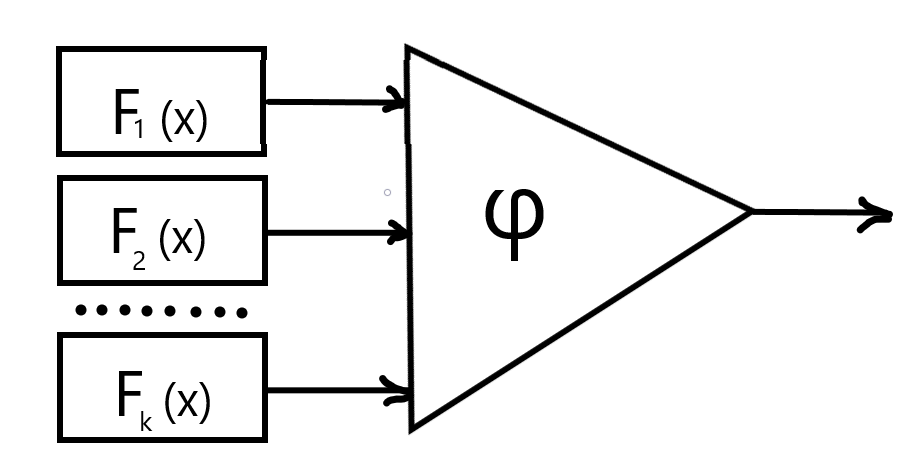
\includegraphics[scale=0.35]{DSC}
\end{figure}

Пусть $F_1, \dots, F_k$ - многочлены попарно взаимопростых степеней $m_1, \dots m_k$.

Тогда,
$$
T=[T(F_1), \dots, T(F_k)] = \frac{(q^{m_1} - 1) \cdot \ldots \cdot (q^{m_k} - 1)}{(q-1)^{k-1}}.
$$

$(q^{m_1} - 1) \cdot \dotsc \cdot (q^{m_k} - 1)$, каждый из них лежит на цикле длины $T$ и таких циклов $(q-1)^{k-1}$ . Будем считать, что начальное состояние $\vec{\alpha_0} = (u_1(0), \dots, u_1(m_1 - i),u_2(0),\dotsc, u_2(m_2-1), \dots, u_k(0), \dots, u_k(m_k-1))$ выбирается из множества $S$ всех состояний, тогда $\vec{\alpha_i}=(u_i(i), \dots, u_i(i+m_1-1), \dots, u_k(i), \dots, u_k(i+m_k-1) \in S$.
Последовательность $((\vec{\alpha_i})_{i=0}^{\infty})$ - чисто периодическая с периодом $T$.
Каждый вектор $\vec{\alpha} \in S$ запишем в виде $\vec{\alpha} = (\vec{\alpha}(1); \dots; \vec{\alpha}(k))$ , где $\vec{\alpha}(j) \in P^{m_j} \textbackslash \{\vec{0}\}$.

Зададим отношение $\sim : \forall \vec{\alpha}, \vec{\beta} \: \vec{\alpha}\sim\vec{\beta} \Leftrightarrow \exists c_1, \dots, c_k \in P^*|\vec{\alpha}(j) = c_j \vec{\beta}(j) \forall j \in \overline{1,k}$

Пусть $a_j$ - корень многочлена $F_j(x)$ в расширении $GF(q^{m_j})$ поля $P$, где $j \in \overline{1,k}$. Из пункта 3 утверждения следует, что $b_j = a_j \frac{q^{m_j}-1}{q-1} = a_j^{T_{red}(F_j)}, i \in \overline{1,k}$ , т.е. имеем мультипликатор многочлена $F_j(x)$ . Пусть $m=m_1; \dots; m_k$, положим $\forall \vec{\alpha}, \vec{\beta} \in S \: \vec{\alpha} \stackrel{red}{\sim} \vec{\beta} \Leftrightarrow \exists i \in \{0, \dots, q-2\} | \vec{\alpha}(j) = \vec{\beta}(j) * b^{m-i/n_j}, \forall j \in \overline{1,k}$ .

Для любого вектора $\exists$ ровно $q-1$ вектор, находящийся с ним в отношении $\stackrel{red}{\sim}$ .

\thr
Пусть $\vec{\gamma_1}, \vec{\gamma_2} \in S$, тогда

1) $\vec{\gamma_1} \sim \vec{\gamma_2}$

2) $\vec{\gamma_1} \bcancel{\stackrel{red}{\sim}} \vec{\gamma_2}$%ну не вот это отношение перечеркнутое типа, вы поняли?

Тогда $\vec{\gamma_1}$ и $\vec{\gamma_2}$ лежат на различных циклах. 
\newpage
% =========================

% ======= Лекция 6 ========
\section{Латинские квадраты}

Для элементов симметрической группы подстановок определим понятие противоречивости.

\opr Подстановки $S$ и $S'$ - противоречивы, если $S(i) \neq S'(i) \forall i \in \overline{1,n}$. Обозначается $S\uparrow S'$.

Определим метрику Хемминга как функцию на множестве $N_m^n = \{ S = S(1), \dotsc,S(n) \mid S(i) \in N_m\}$, где $N_m = \{1, \ldots, m\}$\par
Расстоянием между подстановками назовём $\rho(S',S) = \left|\{i : S(i) \neq S'(i); 
\newline 1 \leq i \leq n\}\right|$
Функция $\rho$ является метрикой Хемминга.

\prop
\begin{enumerate}
	\item $\rho(S,S') \geq 0$ и $\rho(S,S') = 0 \Leftrightarrow S = S'$
	\item $\rho(S,S') = \rho(S',S)$
	\item $\rho(S,S'') \leq \rho(S,S') + \rho(S',S'')$
\end{enumerate}

\utv $S \uparrow S' \Leftrightarrow \rho(S,S')=n$

\opr Последовательноть из $m$ подстановок степени $n$, $2\leq m\leq n,$ обозначаемая \newline$[S_1, S_2, \dotsc, S_m]_n$ образует латинский прямоугольник размеров $m\times n$, если $S_i\uparrow S_j \:\forall i\neq j$.
Любая последовательность из одной подстановки образует латинский прямоугольник размеров $1\times n$.

Если $m=n$, то латинский прямоугольник становится квадратом.

Таблицей латинского прямоугольника $[S_1]_n$ является нижняя строка подстановки $S_1$. \par
В общем случае имеем:
$\begin{pmatrix}
S_1(1) & S_1(2) & \dotsc & S_1(n)\\
S_2(1) & S_2(2) & \dotsc & S_2(n)\\
\vdots & \vdots  & \ddots   & \vdots  \\
S_m(1) & S_m(2) & \dotsc & S_m(n)
\end{pmatrix}$\par

\prop
\begin{enumerate}
	\item В любой строке и любом столбце элементы попарно различны.
	\item В латинском квадрате в любой тройке $(i, j, S_i(j))$ 2 элемента однозначно определяют третий.
\end{enumerate}

$\emph{\textbf{Теорема 1.}}\forall$ латинского прямоугольника $[S_1, \dotsc, S_m]_n;\: 1\leq m < n, \:\exists S_{m+1}\textbar S_{m+1}\uparrow S_i, \: i\in \overline{1,n}$ добавление которой даёт латинский прямоугольник размеров $(m+1)\times n$

$\emph{\textbf{Теорема 2.}}\forall$ латинского прямоугольника $[S_1, \dotsc, S_m]_n$ существует латинский прямоугольник \newline$[S_{m+1}, \ldots, S_n]_n \mid [S_1, \dotsc, S_n]_n$ - латинский квадрат.

\emph{Док-во Теоремы 1:}\par
$\rhd$Рассмотрим семейство подмножеств $(\mathfrak{X}_1,\dotsc,\mathfrak{X}_n)$ множества $\mathfrak{X} = N_n$. Положим $\mathfrak{X}_j = \newline =N_n\setminus\{S_1(j),\dotsc, S_m(j)\}, \: 1\leq j\leq n$. \par
Докажем, что $\exists (x_1, \dotsc, x_n)$ тр. $(\mathfrak{X}_1, \dotsc, \mathfrak{X}_n)$. Т.к. подстановки $S_1, \dotsc, S_m$ попарно противоречивы, то $|\mathfrak{X}_i| = n-m, \: i\in \overline{1,n}$. Рассмотрим мультимножество $(\mathfrak{X}_1, \dotsc, \mathfrak{X}_n)$ с порождающим множеством $\mathfrak{X}$, где $[x_1^{a_1},\dotsc, x_n^{a_n}]$ его первичная спецификация. $\sum\limits_i a_i = n(n-m)$. Покажем, что $\forall i, \: a_i = n-m\: (*)$\par
Зафиксируем $i=1,\dotsc,n\:\forall r=1,\dotsc,m$ однозначно определяется элемент $j_r\in N_n\textbar S_r(j_r)=x_i$, т.к. $S_1, \dotsc, S_m$ попарно противоречивы, то элементы $j_1, \dotsc, j_m$ - попарно различны $\Rightarrow$ по определению $\mathfrak{X}_j, \: x_i\in\mathfrak{X}_{j_r}\: r=1,\dotsc, m; \: x_i\in\mathfrak{X}_j; \notin\{j_1,\dotsc,j_m\}\Rightarrow$ верно (*). \par Покажем, что $(\mathfrak{X}_1,\dotsc, \mathfrak{X}_n)$ удовлетворяет условиям критерия Ф.Холла. Зафиксируем $k\in\overline{1,n}$ и $1\leq j_1<\dotsc<j_k\leq n$. Положим $z=|\mathfrak{X}_{j_1}\cup\dotsc\cup\mathfrak{X}_{j_k}|$. Рассмотрим мультмножества $(\mathfrak{X}_{j_1},\dotsc, \mathfrak{X}_{j_k})$ с порождающим множеством $\mathfrak{X}$, оно включено в большее мультимножество $\mathfrak{X}_1,\dotsc,\mathfrak{X}_n\:(**)$. $[x_1^{a'_1},\dotsc, x_n^{a'_n}]$ - его первичная спецификация, тогда $t'=a'_1+\dotsc+a'_n=k(n-m)$ т.к. (**)$\forall i\in 1,\dotsc,n$ имеет место неравенство $a'_i\leq a_i\Rightarrow a'_i\leq(n-m)$\par
Т.к. $\mathfrak{X}_{j_1}\cup\dotsc\cup\mathfrak{X}_{j_k}$ - носитель мультимножества $(\mathfrak{X}_{j_1}, \dotsc, \mathfrak{X}_{j_k})$, то $z=|\mathfrak{X}_{j_1}\cup\dotsc\cup\mathfrak{X}_{j_k}|=|\{ i\textbar a'_i>0;i\in 1,\dotsc,n\}|\Rightarrow t'=\sum\limits_i a'_i\leq z(n-m)\Rightarrow z\geq k$ и выполянется условие критерия Ф.Холла $\Rightarrow\exists (x_1, \dotsc,x_n)$тр.$(\mathfrak{X}_1, \dotsc,\mathfrak{X}_n)$. Определим $S_{m+1}$ равенством $S_{m+1}(j)=x;\:S_{m+1}\uparrow S_i\:\forall i\in\overline{1,m}$ т.к. $x_j\in N_n\setminus\{S_1(j),\dotsc, S_m(j)\}\triangleleft$

\opr 2 латинских квадрата называются ортогональными, если $\{S_i(j),S'_i(j)\}=N_n\times N_n$, т.е. при наложении таблиц получаем всевозможные пары. 

\thr Если $n$ - нечетное или $n$ делится на 4, то $\exists$ пара ортогональных латинских квадратов порядка $n\times n$

В случае $n$ - нечётное\par
$\left.
\begin{array}{ccc}
	S_i(j)=k\equiv i+j(mod\:n)\\
	S'_i(j)=l\equiv i-j(mod\:n)\\
\end{array}
\right\}(***)$\par
т.к. $n$-нечётное, то $\exists !$ пара $i$ и $j$ удовлетворяющих (***).

\examplei Используется в протокле с разделённым секретом.
\newpage
% =========================

\end{document}
